\documentclass[12pt]{article}
\usepackage{graphicx}
\usepackage{amsmath}
\usepackage{mathtools}
\usepackage{gensymb}
\usepackage[utf8]{inputenc}
\usepackage{float}
\newcommand{\mydet}[1]{\ensuremath{\begin{vmatrix}#1\end{vmatrix}}}
\providecommand{\brak}[1]{\ensuremath{\left(#1\right)}}
\providecommand{\norm}[1]{\left\lVert#1\right\rVert}
\newcommand{\solution}{\noindent \textbf{Solution: }}
\newcommand{\myvec}[1]{\ensuremath{\begin{pmatrix}#1\end{pmatrix}}}
\let\vec\mathbf

\begin{document}
\begin{center}
\textbf\large{CLASS-11 \\ CHAPTER-10 \\ STRAIGHT LINES}
\end{center}
\section*{Excercise 10.4}

Q2. Find the values of $\theta \text{ and } p$, if the equation $x\cos\theta+y\sin\theta=p$ is the normal form
of the line $\sqrt{3}x+y+2=0$.
\\
\solution
\\
From the given line equation:
	\begin{align}
		\vec{m}&=-\sqrt{3}\\
		c&=-2
	\end{align}
        The directional vector is given by:
	\begin{align}
		\vec{m}&=\myvec{1\\-\sqrt{3}\\}
	\end{align}
	The normal vector is given by:
		\begin{align}
	\vec{n}&=\myvec{-\sqrt{3}\\-1\\}\\
	\vec{n}^\top&=\myvec{-\sqrt{3} & -1}
			\end{align}
	Angle between perpendicular and the positive $x$-axis is given by:
		\begin{align}
		\cos\theta&=\frac{\vec{e}_{1}^\top\vec{n}}{\norm{\vec{e}_{1}}\norm{\vec{n}}}\\
			&=\frac{\myvec{1&0\\}\myvec{-\sqrt{3} \\ -1\\}}{2}\\
			&=-\frac{\sqrt{3}}{2}\\
			\implies	\theta&=210\degree
		\end{align}
	The perpendicular distance to the line is given by:
		\begin{align}
			p=\frac{|c|}{\norm{\vec{n}}}=\frac{2}{2}=1
		\end{align}
\begin{figure}[H]
	\begin{center} 
	    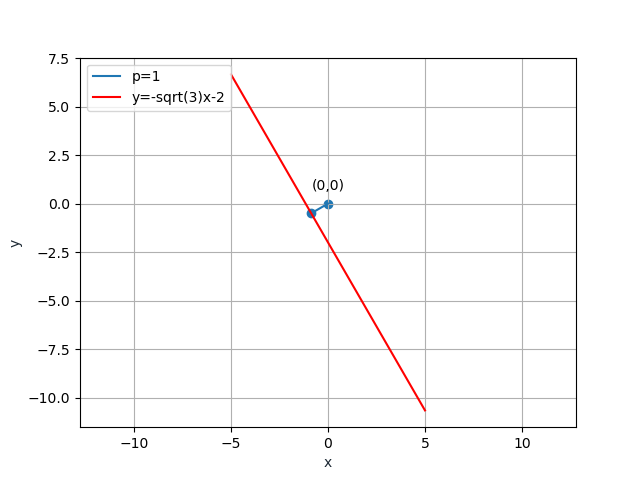
\includegraphics[width=\columnwidth]{figs/line.png}
	\end{center}
\caption{}
\label{fig:Fig1}
\end{figure}
\end{document}